\documentclass[10pt]{report}

%%%%%%%%%%%%%%%%%%%%%%%%%%%%%%%%%%%%%%%%%%%%%%%%%%%%%%%%%%%%%%%%%%%%%%%%%%%%%%%%
% LaTeX Imports
%%%%%%%%%%%%%%%%%%%%%%%%%%%%%%%%%%%%%%%%%%%%%%%%%%%%%%%%%%%%%%%%%%%%%%%%%%%%%%%%
\usepackage{amsfonts}                                                   % Math fonts
\usepackage{amsmath}                                                    % Math formatting
\usepackage{amssymb}                                                    % Math formatting
\usepackage{amsthm}                                                     % Math Theorems
\usepackage{arydshln}                                                   % Dashed hlines
\usepackage{attachfile}                                                 % AttachFiles
\usepackage{cancel}                                                     % Cancelled math
\usepackage{caption}                                                    % Figure captioning
\usepackage{color}                                                      % Nice Colors
\input{./lib/dragon.inp}                                                % Tikz dragon curve
\usepackage[ampersand]{easylist}                                        % Easy lists
\usepackage{fancyhdr}                                                   % Fancy Header
\usepackage[T1]{fontenc}                                                % Specific font-encoding
%\usepackage[margin=1in, marginparwidth=2cm, marginparsep=2cm]{geometry} % Margins
\usepackage{graphicx}                                                   % Include images
\usepackage{hyperref}                                                   % Referencing
\usepackage[none]{hyphenat}                                             % Don't allow hyphenation
\usepackage{lipsum}                                                     % Lorem Ipsum Dummy Text
\usepackage{listings}                                                   % Code display
\usepackage{marginnote}                                                 % Notes in the margin
\usepackage{microtype}                                                  % Niceness
\usepackage{lib/minted}                                                 % Code display
\usepackage{./lib/mlptikz}                                              % Tikz mlp
\usepackage{multirow}                                                   % Multirow tables
\usepackage{pdfpages}                                                   % Include pdfs
\usepackage{pgfplots}                                                   % Create Pictures
\usepackage{rotating}                                                   % Figure rotation
\usepackage{setspace}                                                   % Allow double spacing
\usepackage{subcaption}                                                 % Figure captioning
\usepackage{tikz}                                                       % Create Pictures
\usepackage{tocloft}                                                    % List of Equations
%%%%%%%%%%%%%%%%%%%%%%%%%%%%%%%%%%%%%%%%%%%%%%%%%%%%%%%%%%%%%%%%%%%%%%%%%%%%%%%%
% Package Setup
%%%%%%%%%%%%%%%%%%%%%%%%%%%%%%%%%%%%%%%%%%%%%%%%%%%%%%%%%%%%%%%%%%%%%%%%%%%%%%%%
\hypersetup{%                                                           % Setup linking
    colorlinks=true,
    linkcolor=black,
    citecolor=black,
    filecolor=black,
    urlcolor=black,
}
\RequirePackage[l2tabu, orthodox]{nag}                                  % Nag about bad syntax
\renewcommand*\thesection{\arabic{section}}                             % Reset numbering
\renewcommand{\theFancyVerbLine}{{\arabic{FancyVerbLine}}}              % Needed for code display
\renewcommand{\footrulewidth}{0.4pt}                                    % Footer hline
\setcounter{secnumdepth}{3}                                             % Include subsubsections in numbering
\setcounter{tocdepth}{3}                                                % Include subsubsections in toc
%%%%%%%%%%%%%%%%%%%%%%%%%%%%%%%%%%%%%%%%%%%%%%%%%%%%%%%%%%%%%%%%%%%%%%%%%%%%%%%%
% Custom commands
%%%%%%%%%%%%%%%%%%%%%%%%%%%%%%%%%%%%%%%%%%%%%%%%%%%%%%%%%%%%%%%%%%%%%%%%%%%%%%%%
\newcommand{\nvec}[1]{\left\langle #1 \right\rangle}                    %  Easy to use vector
\newcommand{\ma}[0]{\mathbf{A}}                                         %  Easy to use vector
\newcommand{\mb}[0]{\mathbf{B}}                                         %  Easy to use vector
\newcommand{\abs}[1]{\left\lvert #1 \right\rvert}                       %  Easy to use abs
\newcommand{\pren}[1]{\left( #1 \right)}                                %  Big parens
\newcommand{\comb}[2]{\begin{pmatrix}#1\\#2\end{pmatrix}}               %  Combination syntax
\let\oldvec\vec
\renewcommand{\vec}[1]{\oldvec{\mathbf{#1}}}                            %  Vector Styling
\newtheorem{thm}{Theorem}                                               %  Define the theorem name
\theoremstyle{definition}
\newtheorem{ex}{Example}[section]
\definecolor{bg}{rgb}{0.95,0.95,0.95}
\definecolor{white}{rgb}{1, 1, 1}
\newcommand{\java}[4]{\vspace{10pt}\inputminted[firstline=#2,
                                 lastline=#3,
                                 firstnumber=#2,
                                 gobble=#4,
                                 frame=single,
                                 label=#1,
                                 bgcolor=bg,
                                 linenos]{java}{#1}}
\newcommand{\python}[4]{\vspace{10pt}\inputminted[firstline=#2,
                                 lastline=#3,
                                 firstnumber=#2,
                                 gobble=#4,
                                 frame=single,
                                 label=#1,
                                 bgcolor=bg,
                                 linenos]{python}{#1}}
\newcommand{\js}[4]{\vspace{10pt}\inputminted[firstline=#2,
                                 lastline=#3,
                                 firstnumber=#2,
                                 gobble=#4,
                                 frame=single,
                                 label=#1,
                                 bgcolor=bg,
                                 linenos]{js}{#1}}
\newcommand{\json}[4]{\vspace{10pt}\inputminted[firstline=#2,
                                 lastline=#3,
                                 firstnumber=#2,
                                 gobble=#4,
                                 label=#1,
                                 bgcolor=white,
                                 linenos]{json}{#1}}
%%%%%%%%%%%%%%%%%%%%%%%%%%%%%%%%%%%%%%%%%%%%%%%%%%%%%%%%%%%%%%%%%%%%%%%%%%%%%%%%
% Beginning of document items - headers, title, toc, etc...
%%%%%%%%%%%%%%%%%%%%%%%%%%%%%%%%%%%%%%%%%%%%%%%%%%%%%%%%%%%%%%%%%%%%%%%%%%%%%%%%
\pagestyle{fancy}                                                       %  Establishes that the headers will be defined
\fancyhead[LE,LO]{CSCI 3308 Project Proposal}                                  %  Adds header to left
\fancyhead[RE,RO]{Farmer, Maton}                                        %  Adds header to right
\cfoot{\mlptikz[size=0.25in, text=on, textposx=0, textposy=0, textvalue=\thepage, textscale=0.75in]{applejack}}
\lfoot{CSCI 3308}
\rfoot{Stafford}
\title{Project Proposal}
\author{William Farmer\\
        Edward Maton}

%%%%%%%%%%%%%%%%%%%%%%%%%%%%%%%%%%%%%%%%%%%%%%%%%%%%%%%%%%%%%%%%%%%%%%%%%%%%%%%%
% Beginning of document items - headers, title, toc, etc...
%%%%%%%%%%%%%%%%%%%%%%%%%%%%%%%%%%%%%%%%%%%%%%%%%%%%%%%%%%%%%%%%%%%%%%%%%%%%%%%%
\begin{document}

\maketitle

\tableofcontents    % Table of contents
\newpage

\listoffigures      % List of Figures
\newcommand{\listequationsname}{\Large{List of Equations}}          % Funky code to include LOE
\newlistof{myequations}{equ}{\listequationsname}
\newcommand{\myequations}[1]{%
\addcontentsline{equ}{myequations}{\protect\numberline{\theequation}#1}\par}
\listofmyequations

\newpage
%%%%%%%%%%%%%%%%%%%%%%%%%%%%%%%%%%%%%%%%%%%%%%%%%%%%%%%%%%%%%%%%%%%%%%%%%%%%%%%%
% Beginning of content
%%%%%%%%%%%%%%%%%%%%%%%%%%%%%%%%%%%%%%%%%%%%%%%%%%%%%%%%%%%%%%%%%%%%%%%%%%%%%%%%
\begin{abstract}
    This study shows how a ranking system can be applied to Twitter and give a ranking for users based on their influence. Through application of matrix methods, users on Twitter were ranked according to retweets, followers, and favorites. The ranking system was based on the application of the Perron-Frobenius theorem as well as an iterative method. For this particular study, a smaller data set was used due to the complexity of the ranking system as the matrices increase in size. A larger data set would also be hard to model because some users are hardly connected to twitter and don't have much information. Their data might skew the system unless a significantly large data set is analyzed. The first step was to verify the matrix was irreducible. Once the matrix was found to be irreducible, the Perron-Frobenius theorem allowed for the matrix to be manipulated with an iterative method. Traditional power iteration was used for approximation of the dominant eigenvector, and was able to determine an accurate ranking for our users.

\end{abstract}

\section{Introduction}
Twitter is a free, online social media website with over 550 million users worldwide. It allows a user to create brief messages, or ``tweets'' (not exceeding 140 characters in length), and share them with their followers. The popularity of this website has greatly altered the way in which information is transferred across the world, as well as the speed at which this is done. With that being said, any one user has the opportunity to become rather influential based on how many other users on Twitter interact with his/her tweets. Because of its clear relevance in the modern world, celebrities, bloggers, and news media sites have taken to sharing information with Twitter. Some especially famous celebrities have several millions of followers, and are obviously incredibly influential in the world of Twitter.

    We then seek to rank Twitter users based on how influential they are to other users. In order to do so, one must account for the three most common forms of interaction on the website: followers, favorites, and retweets.

        To understand these three interactions, take for example user A and user B. If user A ``follows'' user B on Twitter, anything that user A tweets will appear on user B's news feed. This is by far the most common form of interaction. If user A ``favorites'' a tweet from user B, user A expresses his/her interest in user B's tweet because of its humor, importance, relevance, etc. Users can see one another's favorited tweets, so if user B is commonly favorited there is a good chance others will see his/her tweets. Finally, the least common interaction, a ``retweet'' occurs when user B chooses to allow a tweet from user A to show on his/her page. In doing so, all of the followers of user B see the tweet that user A posted. This broadens the scope of their influence, as many more followers are able to see the tweet without having to search for it. This can quickly allow a tweet from someone with a small amount of followers to reach a large amount of users.

                Due to the immense amount of users in Twitter, an analysis of the entire population would be very time consuming and difficult. We therefore limit the scope of our analysis to a random sample of tweets in the Boulder area. However, since these tweets could be retweets of users outside of Boulder, or even the country, our data set will almost certainly include a broad spectrum of users.


\section{Materials and Methods}
    Because there was a large amount of data that needed to be analyzed, there were numerous tools that were necessary for an effective study. The tools used include Twitter's development API as well as programming methods for analysis of the data. The first step to figuring out the ranking was to obtain the data from twitter that needed to be analyzed. Twitter's development API allowed us to take the necessary data in order to rank the users, which included the tweets of different users as well as many crucial details about the user's account. For the ranking method used, the only tweets that were needed were the, relatively rare, retweets to allow for a more accurate ranking. The idea behind it was that it took out any data that could be considered an outlier, as well as limit our search to users that were actually important enough to be retweeted.

Once the data from Twitter was acquired through the API, the tweets needed to be processed in a way that the ranking method could then be applied. Doing the work by hand would have been nearly impossible due to the amount of data and the complexity of the ranking methods.\footnote{Our final network had 2715 individual users.} In order to analyze the data effectively we needed to use more sophisticated data analytical tools. Python, R and SQL were the three main languages used for the analysis, with Python being predominant due to its all-purpose intent as well as its relatively simple syntax and library support. It also handles Twitter nicely using {\ttfamily requests} and {\ttfamily requests\_oauthlib} to manage their OAuth authentication system. R was used primarily because of its support of larger filebacked matrices, but also because it can handle large data sets and has built in tools for visualization. We chose to store the raw data in a SQLite database, which is very easy to use with both Python as well as R, because of it's inherent connectability between the different languages as well as its relatively lightweight framework. With those three tools, the ranking method could then be applied to the Twitter data.

In terms of use, Python was used solely to obtain the data from Twitter's API and create the visualizations. Once the data was stored, a primary ranking algorithm was established to determine edge weights in our network. There were three criteria in our ranking algorithm which were the number of followers, the favorites and the retweets.

    \begin{equation}\label{eq:influence}
        Influence=x \cdot (followers)+y \cdot (favorites)+z \cdot (retweets)
    \end{equation}\myequations{User Influence}

We decided that because retweets were so rare, they would carry the most weight for our influence score. Followers and favorites were fairly common on Twitter so they didn't carry as much importance. In this study, for the above equation, $x=1,y=1,z=8$.\footnote{Note, it would be trivial to adjust this influence equation and determine a different ranking based on a different numerical meaning of ``influence''} Once our parameters were obtained, the ranking algorithm we created was applied using R. The application of our ranking algorithm gave us an adjacency matrix\footnote{It is important to note at this time that the edges were established from (most importantly) retweets and follower links. Every retweet was given an edge weight of $ 8 \cdot retweets + nodeweight $, and every follower was given a weight of $ follower * nodeweight $. Follower edges were only added if the user that was being followed existed within the established dataset, and retweet edges, by nature had to exists within the dataset.}, which was then normalized to give us our stochastic matrix. One theorem that was necessary to verify we could proceed was the Perron-Frobenius theorem which states that a real square matrix with positive entries has a unique largest real eigenvalue and that the corresponding eigenvector has strictly positive components. The Perron-Frobenius theorem also required our matrix be irreducible, which allowed us to proceed with finding the ranks. The last step for obtaining our final ranks was to apply the power iteration method, and thusly obtain an approximation of our dominant eigenvector.

    \subsection{Analysis Overview}
    There were four main steps involved in analysis.\footnote{For a more complete and helpful diagram, please see Appendix~\ref{app:workflow}.}

        \NewList
        \begin{easylist}[enumerate]
            & Data Acquisition and Formatting (Python)
            & Data Cleaning (Python)
            & Data Entry (R)
            & Analysis (R)
        \end{easylist}

    \subsection{Data Acquisition and Formatting}
    The first step of this process was to import the data from Twitter's streaming API.

        \python{./code/twitterImport.py}{21}{25}{4}

    Twitter provides a handy url for streaming a random subset of all Twitter traffic. In order to avoid overfitting, or selection bias we used this random subset for all data analysis. We limited our search to English posts from Boulder, CO in order to hopefully acquire a densely connected network of related posts.

    The next step is to either create the SQLITE database or open a previously existing one. The tables in the database are created with the following python code, and look like Table~\ref{table:database-tables}.

        \python{./code/twitterImport.py}{29}{44}{8}

        \begin{table}[ht]
            \centering
            \begin{tabular}{| l | l | l |}
                \hline
                \textbf{users} & \textbf{posts} & \textbf{retweets}\\
                \hline
                id (text) & id (text) & id (text)\\
                \hline
                name (text) & time (text) & end (text)\\
                \hline
                followers (text) & entities (text) & count (int)\\
                \hline
                favourites\_count (int) & user (text) & \\
                \hline
                followers\_count (int) & & \\
                \hline
                friends\_count (int) & & \\
                \hline
            \end{tabular}
            \caption{Database Tables}
            \label{table:database-tables}
        \end{table}

    Once our database has been established, we move on to the actual data import process. The code block below shows the steps in the order they are completed. For a more detailed reference, please see the attached source code.

        \python{./code/twitterImport.py}{61}{65}{4}

    After this has been completed we have a full database filled with many unique users and posts.

    \subsection{Data Cleaning}
    After our initial data has been imported, we need to clean the data. In order for our analysis method to work, we need to acquire an irreducible\footnote{Irreducible in this case meaning that all nodes are connected to each other, and the matrix cannot be split into two or more adjacency matrices} adjacency matrix.\footnote{Where an adjacency matrix is the matrix representation of our network of users connected by retweets}. The first step is to establish a new database entirely using the name of the previous database. The structure of this new database is identical to the old, save it is missing the posts table.

    After the database is established, we scan our old database and do three things:

        \NewList
        \begin{easylist}[enumerate]
            & Find the \textit{most important} user. This is determined by who has the most edges (retweets) connecting them to the other users.
            & Find all users that have an edge between them and the most important user.
            & Recursively apply step 2 to obtain the complete network.
        \end{easylist}

    Step 1 is accomplished by aggregating the retweet table into absolute scores counting how many times a user was retweeted. The user with the most retweets is defined as our ``most important user'' and only connected users are added to the clean database.

        \python{./code/pyRank.py}{108}{121}{4}

    All users connected to our important user are then added to the new database by looping through user addition until the network no longer changes size from one iteration to the next.

        \python{./code/pyRank.py}{123}{143}{4}

    This then gives us a list of all users connected to the most important user, as well as the most important user itself. We then iterate through the old database and copy all relevant information from the old database to the new one if and only if the user exists in our list of connected/important users. At this point the data has been cleaned and all further analysis will be performed on the clean database.

    \subsection{Data Entry}
    Now that we have a reliable data source, we can analyze the data. This is accomplished using the R language. R is very good at handling large quantities of data, and as a result is ideal for this situation. The R code for the analysis is contained in {\ttfamily ./code/ranking.R}, and can be run separately from the python program, however this is not recommended.

    The first step to importing the data from our previously established clean SQLITE database is to create the user dataframe.\footnote{In R, a dataframe is a special datatype that is useful for many applications. For more information, I would recommend \url{http://stat.ethz.ch/R-manual/R-devel/library/base/html/data.frame.html}} As part of this operation, we need to establish a list of users by querying the user table from our clean database.

    \rlang{./code/ranking.R}{16}{24}{0}

    Once we have our list of users, we can then construct the dataframe by finding the weight of the user from individual database queries.

    \rlang{./code/ranking.R}{26}{48}{0}

    This dataframe construction gives us the following dataframe. Please see Appendix~\ref{app:userweights}  to see a more complete dataframe.

        \begin{equation}\label{eq:userdataframe}
            \begin{pmatrix}
              390267816 & 2349.00 \\ 
              1167483505 & 33.00 \\ 
              853887943 & 34.00 \\ 
              325869713 & 1798.00 \\ 
              898986895 & 902.00 \\ 
              1328457397 & 1616.00 \\ 
              1355302483 & 721.00 \\ 
              1266058160 & 3682.00 \\ 
              515334031 & 366.00 \\ 
              230436012 & 1082.00 \\ 
              371462259 & 1946.00 \\ 
              298627315 & 2740.00 \\ 
              449047486 & 5743.00 \\ 
              630746058 & 11330.00 \\ 
              1143867078 & 4359.00 \\ 
              461854939 & 87.00 \\ 
              707394641 & 653.00 \\ 
              204178374 & 328.00 \\ 
              454467056 & 648.00 \\ 
              1740729596 & 1406.00 \\ 
              555636619 & 1183.00 \\ 
              783648271 & 2189.00 \\ 
              582951657 & 7693.00 \\ 
              216346618 & 659.00 \\ 
              1656121652 & 1304.00 \\ 
              714914388 & 4165.00 \\ 
              1370674644 & 2044.00 \\ 
              341134422 & 1336.00 \\ 
              580051343 & 6002.00 \\ 
              1451680514 & 3076.00 \\ 
            \end{pmatrix}
        \end{equation}\myequations{Abbreviated User-Weight Dataframe}

    Now that we have our user weights dataframe, we can determine the links between users, and construct yet another dataframe consisting of all follower links between our users.

    \rlang{./code/ranking.R}{50}{61}{0}

    We finally have all the information we need in the correct formats in order to create our matrix. Four separate functions are referenced in order to optimize our code for speed. These functions are described below.

    \rlang{./code/ranking.R}{71}{98}{0}

        \subsubsection{Create Matrix}
        \rlang{./code/ranking.R}{63}{69}{0}

        This generates an $n \times n$ filebacked matrix to be populated later.

        \subsubsection{Replace}
        \rlang{./code/ranking.R}{122}{135}{0}

        Replace takes each row in our SQL query and adds a link from retweets in our adjacency matrix in the correct position.

        \subsubsection{Followers}
        \rlang{./code/ranking.R}{100}{120}{0}

        Followers takes each row in our SQL query and adds a link from followers in our adjacency matrix in the correct position.

        \subsubsection{Normalize}
        \rlang{./code/ranking.R}{137}{145}{0}

        Normalize replaces each row with the row divided by its sum. This gives us a probability matrix.

    \subsection{Analysis}
    In order to determine the rankings of the users, we first construct an arbitrary vector with length equal to the number of users with unit length 1. Our non-orthonormalized matrix is of the form

        \begin{equation}\label{matrix:startingA}
            \begin{pmatrix}
                1\\
                1\\
                1\\
                \vdots\\
                1
            \end{pmatrix}
        \end{equation}\myequations{Initial Arbitrary Vector}

    We then pass the vector and matrix to our power method which runs however many iterations are specified. Please see the beginning of this section for more explanation on how the algorithm works.

    \rlang{./code/ranking.R}{151}{159}{0}

    These two steps will run as many times as specified, and when complete (or nearly so) they will give us an approximation to our eigenvector. This eigenvector has a direct one-to-one correspondence to our user's relative rank compared to this network.


\subsection{Analysis}
    Using the data available we were able to successfully rank the users on their relative influence compared to the selected group. In~\ref{eq:eigenvector} we only have 26 non-zero values in our approximated eigenvector. Our full results can be found in Appendix~\ref{app:results}

\begin{equation}\label{eq:eigenvector}
    \left\{
        \underbrace{%
            \begin{pmatrix}
                14\\
                21\\
                23\\
                32\\
                33\\
                34\\
                42\\
                52\\
                53\\
                57\\
                61\\
                65\\
                68\\
                69\\
                76\\
                88\\
                89\\
                100\\
                102\\
                114\\
                116\\
                117\\
                155\\
                1018\\
                1457\\
                2692\\
            \end{pmatrix}
        }_{\text{Index}}
        \underbrace{%
            \begin{pmatrix}
                6.64949232632148e-06\\
                1.09911011888071e-05\\
                11.855584902313\\
                0.000579864962983945\\
                0.000151203180869463\\
                5.66269756293866e-05\\
                3.43608910353295e-06\\
                0.000207441307238603\\
                0.000596997173695231\\
                6.64949232632148e-06\\
                5.53795798073443\\
                0.00014002408432437\\
                0.000579864962983945\\
                0.000810638056052665\\
                0.000108830685549892\\
                11.8555814662239\\
                0.000105152995730235\\
                0.000171495791986021\\
                5.27313420768053e-05\\
                3.43608910353295e-06\\
                3.43608910353295e-06\\
                5.95354325766195e-05\\
                22.8520643143014\\
                0.000596997173695231\\
                0.000207595719100648\\
                1.36186831565854e-05\\
            \end{pmatrix}
        }_{\text{Value}}
    \right\}
\end{equation}\myequations{Resulting Eigenvector}

If you'll note, the user with the highest score is user 155, which correspondes to Twitter user 27260086. This user's screen name is ``justinbieber''.

Looking at our user connections we can start to determine what our graph looks like. We have one central user that has many connections leading to him, however we also have many other users that contribute solely to other users, and often aren't related to our ``main'' user at all. These users are often dissacociated from our main user by at least one degree, and we have up to four degrees of separation when you look at our furthest distant user.

\begin{figure}[ht]
    \centering
    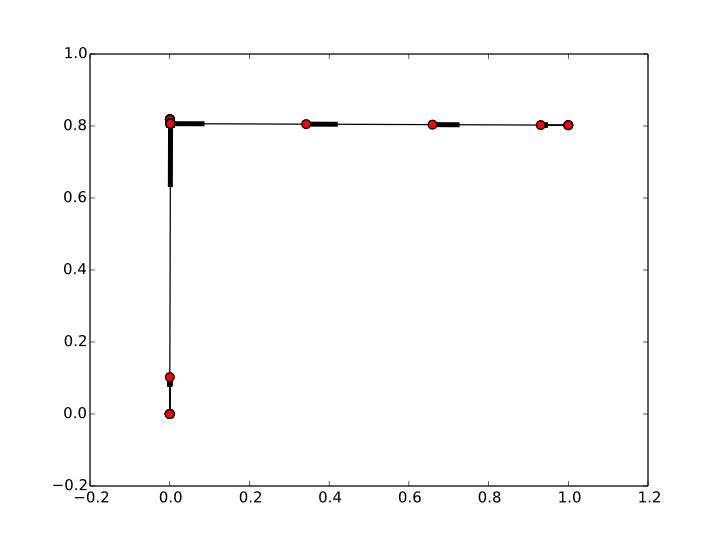
\includegraphics[scale=0.8]{./img/links.png}
    \caption{Simplified Links of our Established Network}
    \label{fig:links}
\end{figure}

If we look at the entire expanded network we see a similar picture. Our users are clustered around one main user, and it is obvious that the network has one focal point, however when examined closely it becomes apparent that some users have no connections to our main user and instead point to just one sub-user instead.

\begin{figure}[ht]
    \centering
    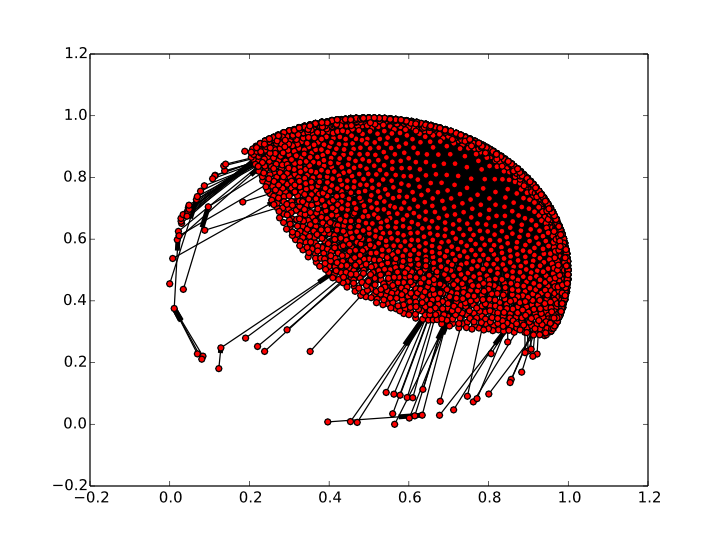
\includegraphics[scale=0.8]{./img/users.png}
    \caption{All Users of our Established Network}
    \label{fig:users}
\end{figure}

Given our results these networks make intuitive sense; we have one user that is focused upon, and everyone else is of little to no importance. When looking at Twitter's population this result begins to hold true for a large portion of Twitter users. Most users are either fairly passive or of too little consequence to be highlighted.


\section{Conclusion}

    \subsection{Implications}
        Aside from friends being able to look at one another's popularity, our analysis offers assistance in several different fields. Most prominently, advertising companies could utilize the ranking to find the most influential Twitter users and work with them to reach as many people as possible. Since every interaction on Twitter is available to everyone with their development system, anyone could perform similar analysis to ours.

As a company, Twitter could even find this process useful. Being able to find their most active users would be an incredibly useful tool for analysis of the functionality of the website. While we only sampled a very small subset of users, Twitter could include and compute the ranking with every user in the data set--something even more valuable.

Beyond these uses, an interesting abstract idea is the thought that due to applications of matrix methods, one can literally assign a human a ranking of influence. While not everyone in the world uses Twitter and our definition of influence is not absolute, it is still peculiar that an entire population can be ranked by popularity with ease, despite a large data set.

A simplistic demonstration of this potential service is available at \url{www.will-farmer.com/twilight}. This website was created by William Farmer, and uses a simplified algorithm to rank the users.


    \subsection{Discussion}
        After implementing the power method and isolating the final dominant eigenvector, we had an explicit ranking of the users in our data set. An interesting note in this eigenvector was the large amount of users with negligible influence; out of nearly 3000 users, only 26 had an influence value greater than zero. This did not come as too much of a surprise due to the nature of our sample data set. Many of these users likely retweeted one of the more influential people and had no other interactions, diminishing their relative influence.

This clear difference in number of users with appreciable influence and those with almost no influence imply that the vast majority of users on Twitter are not all that influential. Our data suggests that in fact there are very few users who truly hold significant weight. As a matter of fact, we found one of the influential users in our data set was none other than Justin Bieber. While he does not live in Boulder, several people must have retweeted him and thereby introduced him to our data set. With his some 47 million followers, it does not come as a surprise that he was one of the most influential users on Twitter in our analysis.

This does relay a rather dismal message to almost the entire remainder of Twitter users however--they are just not that important. With the massive amount of followers and retweets that celebrities like Justin Bieber have, it is highly unlikely that a random user's tweets will reach the majority of the users on Twitter. However, this will certainly not keep people from using Twitter. Many users have an account simply to follow celebrities or comedians. Other have one to keep up with their sports teams or local news stations. Having a Twitter account is not always about trying to be the most popular user. Instead, it serves as a means of quick and easy communication for friends and celebrities alike.


\newpage

\appendix

\section{Workflow}\label{app:workflow}
    \begin{figure}[ht]
        \centering
        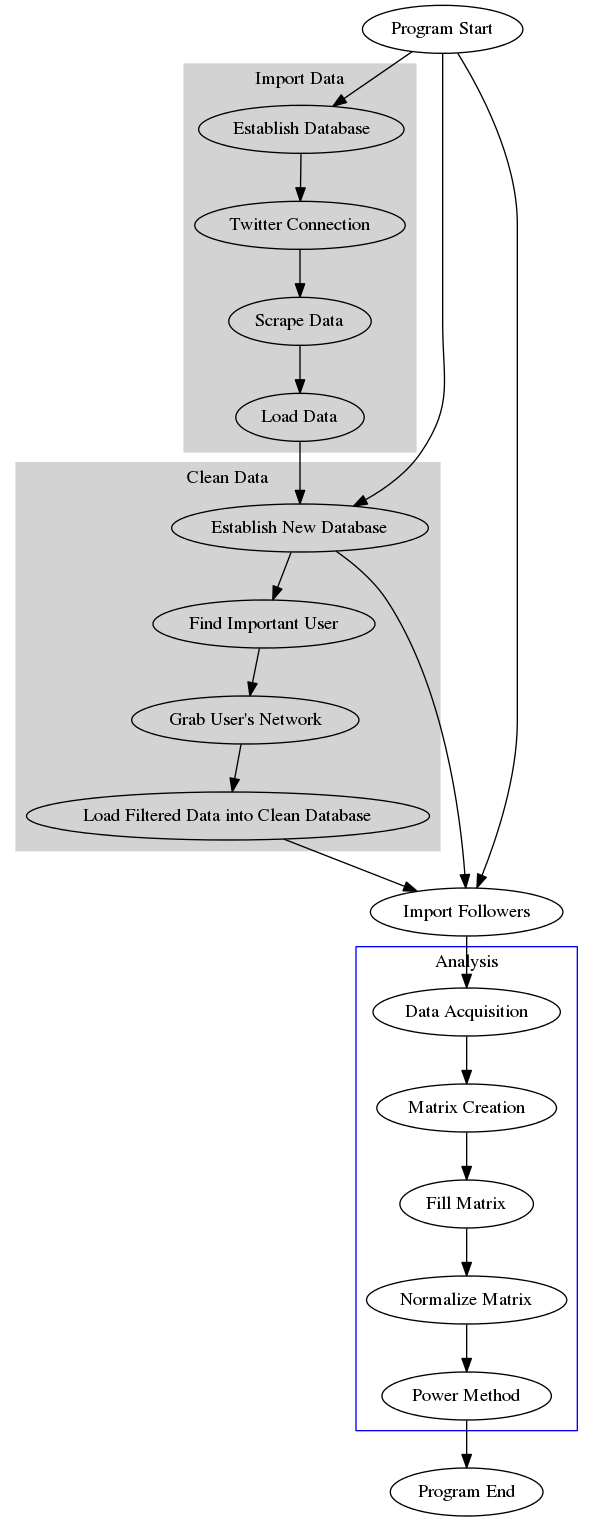
\includegraphics[scale=0.3]{./img/flow.png}
        \label{img:flow}
        \caption{Workflow Diagram}
    \end{figure}

\section{Eigenvector}\label{app:results}
Our .csv eigenvector can be found \attachfile{./code/eigenvector.csv}{here}.

\section{User Weight Dataframe}\label{app:userweights}
Only users with a weight greater than 10,000 have been shown. For a full listing, please download \attachfile{./code/fulldataframe.csv}{User Weights}.
% latex table generated in R 3.0.2 by xtable 1.7-1 package
% Fri Dec 13 00:02:52 2013
\twocolumn
\begin{centering}
\tablehead{%
    \hline
    Index & User & Weight\\
    \hline
}
\tabletail{%
    \hline
}
\begin{supertabular}{|c|c|c|}
  14 & 630746058 & 11330.00 \\ 
  34 & 326405936 & 10767.00 \\ 
  42 & 624400312 & 12045.00 \\ 
  51 & 564366503 & 13193.00 \\ 
  61 & 94794703 & 11244.00 \\ 
  90 & 186963547 & 19042.00 \\ 
  112 & 327089971 & 16478.00 \\ 
  117 & 540112867 & 10525.00 \\ 
  120 & 411679941 & 10467.00 \\ 
  122 & 970302428 & 35038.00 \\ 
  127 & 609521711 & 21402.00 \\ 
  128 & 100131802 & 11997.00 \\ 
  145 & 634976070 & 28744.00 \\ 
  146 & 106689852 & 14948.00 \\ 
  155 & 27260086 & 47171703.00 \\ 
  159 & 341911569 & 21805.00 \\ 
  179 & 1159366760 & 11572.00 \\ 
  192 & 921812846 & 11562.00 \\ 
  200 & 599747318 & 11904.00 \\ 
  228 & 229478749 & 10904.00 \\ 
  261 & 511016804 & 14763.00 \\ 
  263 & 712518012 & 28174.00 \\ 
  276 & 452386369 & 33685.00 \\ 
  279 & 1663040792 & 10516.00 \\ 
  293 & 1546396718 & 11648.00 \\ 
  322 & 554499917 & 23350.00 \\ 
  324 & 35471715 & 12698.00 \\ 
  334 & 342297272 & 13392.00 \\ 
  389 & 233757681 & 14670.00 \\ 
  425 & 303852627 & 17833.00 \\ 
  433 & 339153652 & 16946.00 \\ 
  436 & 760144261 & 13995.00 \\ 
  464 & 272219232 & 13412.00 \\ 
  465 & 415096035 & 10355.00 \\ 
  493 & 251328265 & 13418.00 \\ 
  508 & 387980396 & 14130.00 \\ 
  526 & 281816610 & 10467.00 \\ 
  527 & 1049301990 & 13737.00 \\ 
  534 & 249763046 & 19570.00 \\ 
  544 & 334612319 & 21648.00 \\ 
  552 & 1462426686 & 18719.00 \\ 
  559 & 1096938487 & 12634.00 \\ 
  571 & 884698502 & 72336.00 \\ 
  601 & 1191641258 & 10118.00 \\ 
  645 & 261267312 & 12640.00 \\ 
  667 & 701679588 & 60758.00 \\ 
  681 & 344123447 & 10241.00 \\ 
  689 & 333962617 & 17114.00 \\ 
  713 & 1054943286 & 17851.00 \\ 
  719 & 806434044 & 13066.00 \\ 
  755 & 136494576 & 13272.00 \\ 
  769 & 379477396 & 12866.00 \\ 
  823 & 1152077396 & 16730.00 \\ 
  835 & 1370034217 & 10423.00 \\ 
  841 & 273177183 & 15853.00 \\ 
  848 & 134300287 & 17914.00 \\ 
  857 & 228034203 & 17240.00 \\ 
  859 & 1628657935 & 11793.00 \\ 
  901 & 1253343157 & 10403.00 \\ 
  903 & 156449730 & 26229.00 \\ 
  914 & 425369749 & 14645.00 \\ 
  919 & 251670427 & 29269.00 \\ 
  923 & 349161702 & 12209.00 \\ 
  948 & 423893401 & 10675.00 \\ 
  950 & 302028075 & 10678.00 \\ 
  957 & 725168408 & 14443.00 \\ 
  964 & 98008008 & 15278.00 \\ 
  976 & 329264315 & 24567.00 \\ 
  979 & 1267870554 & 86059.00 \\ 
  996 & 716045551 & 16734.00 \\ 
  1010 & 548569720 & 11015.00 \\ 
  1021 & 405197592 & 13711.00 \\ 
  1026 & 364363813 & 10473.00 \\ 
  1030 & 223181418 & 257578.00 \\ 
  1041 & 155871002 & 21075.00 \\ 
  1065 & 1411164529 & 19633.00 \\ 
  1073 & 254761626 & 11840.00 \\ 
  1075 & 99368285 & 11159.00 \\ 
  1079 & 277459459 & 13662.00 \\ 
  1082 & 43992418 & 20170.00 \\ 
  1090 & 1231287487 & 11075.00 \\ 
  1091 & 241127563 & 16494.00 \\ 
  1100 & 711021564 & 16203.00 \\ 
  1108 & 465144648 & 14484.00 \\ 
  1119 & 489746004 & 51657.00 \\ 
  1146 & 31775600 & 133275.00 \\ 
  1165 & 502141732 & 27772.00 \\ 
  1170 & 946608667 & 140350.00 \\ 
  1181 & 1177058718 & 11267.00 \\ 
  1195 & 275192872 & 45550.00 \\ 
  1210 & 630470363 & 11932.00 \\ 
  1211 & 508786354 & 15920.00 \\ 
  1251 & 101854971 & 14403.00 \\ 
  1289 & 1061740729 & 24610.00 \\ 
  1294 & 174465013 & 13857.00 \\ 
  1300 & 1011329257 & 11241.00 \\ 
  1304 & 860230987 & 11241.00 \\ 
  1341 & 551246662 & 13501.00 \\ 
  1343 & 40347131 & 11357.00 \\ 
  1358 & 549484617 & 22568.00 \\ 
  1359 & 574715600 & 25299.00 \\ 
  1362 & 336859526 & 14243.00 \\ 
  1384 & 794528744 & 18068.00 \\ 
  1387 & 224921031 & 18339.00 \\ 
  1388 & 124264446 & 10107.00 \\ 
  1414 & 126433456 & 16746.00 \\ 
  1416 & 475655739 & 13170.00 \\ 
  1448 & 157712893 & 17453.00 \\ 
  1449 & 1157273696 & 14516.00 \\ 
  1457 & 585786517 & 19082.00 \\ 
  1485 & 775832820 & 12645.00 \\ 
  1508 & 334384978 & 10991.00 \\ 
  1521 & 441491566 & 11127.00 \\ 
  1524 & 457618957 & 10121.00 \\ 
  1535 & 255645831 & 23107.00 \\ 
  1578 & 634994358 & 47900.00 \\ 
  1582 & 327487739 & 12857.00 \\ 
  1591 & 1063040520 & 39343.00 \\ 
  1596 & 102961107 & 27764.00 \\ 
  1608 & 162800521 & 11485.00 \\ 
  1612 & 144684377 & 25852.00 \\ 
  1619 & 436346220 & 10792.00 \\ 
  1698 & 251323953 & 10697.00 \\ 
  1702 & 946589106 & 12424.00 \\ 
  1777 & 302081484 & 10850.00 \\ 
  1789 & 611843107 & 13880.00 \\ 
  1796 & 878402719 & 26858.00 \\ 
  1824 & 211530541 & 13620.00 \\ 
  1853 & 310640211 & 27623.00 \\ 
  1857 & 1664339594 & 26089.00 \\ 
  1876 & 336809891 & 43156.00 \\ 
  1884 & 465972676 & 30061.00 \\ 
  1911 & 28842209 & 13711.00 \\ 
  1919 & 439269298 & 12527.00 \\ 
  1923 & 1148452152 & 10959.00 \\ 
  1926 & 370383777 & 17931.00 \\ 
  1933 & 1106839123 & 11395.00 \\ 
  1966 & 99172004 & 13172.00 \\ 
  1983 & 741571238 & 16967.00 \\ 
  1985 & 184832093 & 11345.00 \\ 
  1986 & 303138113 & 38332.00 \\ 
  2026 & 1160060478 & 14318.00 \\ 
  2073 & 351169230 & 10909.00 \\ 
  2091 & 135682030 & 13102.00 \\ 
  2092 & 768007074 & 10869.00 \\ 
  2096 & 478087852 & 10064.00 \\ 
  2109 & 569249586 & 11391.00 \\ 
  2117 & 1508402305 & 11422.00 \\ 
  2119 & 235746080 & 12850.00 \\ 
  2124 & 373361072 & 22091.00 \\ 
  2140 & 731538752 & 26125.00 \\ 
  2156 & 1340799422 & 10541.00 \\ 
  2197 & 353451876 & 29308.00 \\ 
  2238 & 1591908384 & 14157.00 \\ 
  2290 & 188971014 & 11325.00 \\ 
  2324 & 110328199 & 18428.00 \\ 
  2347 & 306343981 & 12405.00 \\ 
  2364 & 790831482 & 23295.00 \\ 
  2374 & 1772231389 & 10633.00 \\ 
  2402 & 534633467 & 24961.00 \\ 
  2437 & 624785810 & 13959.00 \\ 
  2448 & 164465678 & 12599.00 \\ 
  2454 & 571239776 & 14849.00 \\ 
  2455 & 705288404 & 15074.00 \\ 
  2457 & 329486211 & 11534.00 \\ 
  2463 & 608724448 & 12165.00 \\ 
  2468 & 787472516 & 15487.00 \\ 
  2480 & 225080589 & 10576.00 \\ 
  2505 & 411006479 & 29723.00 \\ 
  2509 & 184891657 & 12073.00 \\ 
  2513 & 238775866 & 20700.00 \\ 
  2525 & 84546155 & 16784.00 \\ 
  2543 & 406328788 & 17930.00 \\ 
  2553 & 275733498 & 12932.00 \\ 
  2603 & 558826929 & 11854.00 \\ 
  2640 & 397514527 & 11000.00 \\ 
  2664 & 217578833 & 14439.00 \\ 
  2667 & 433687416 & 14952.00 \\ 
  2687 & 797115074 & 25631.00 \\ 
  2692 & 1345120957 & 25628.00 \\ 
\end{supertabular}
\end{centering}
\onecolumn


\section{Attachments}
\attachfile{./tex/attachments.tar.gz}{Report \LaTeX}

\attachfile{./tex/code.tar.gz}{Report Programs}

\section{Authors}
If you have any questions about methods used, are unable to access attached files, or wish to discuss the report more with the authers, please email \url{willzfarmer@gmail.com} or visit \url{www.will-farmer.com} where this paper will be posted.

\end{document}
